\subsubsection{Poziom 1}
\clearpage
\begin{figure}[H]
	\centering
	\vspace{-2cm}
	\centerline{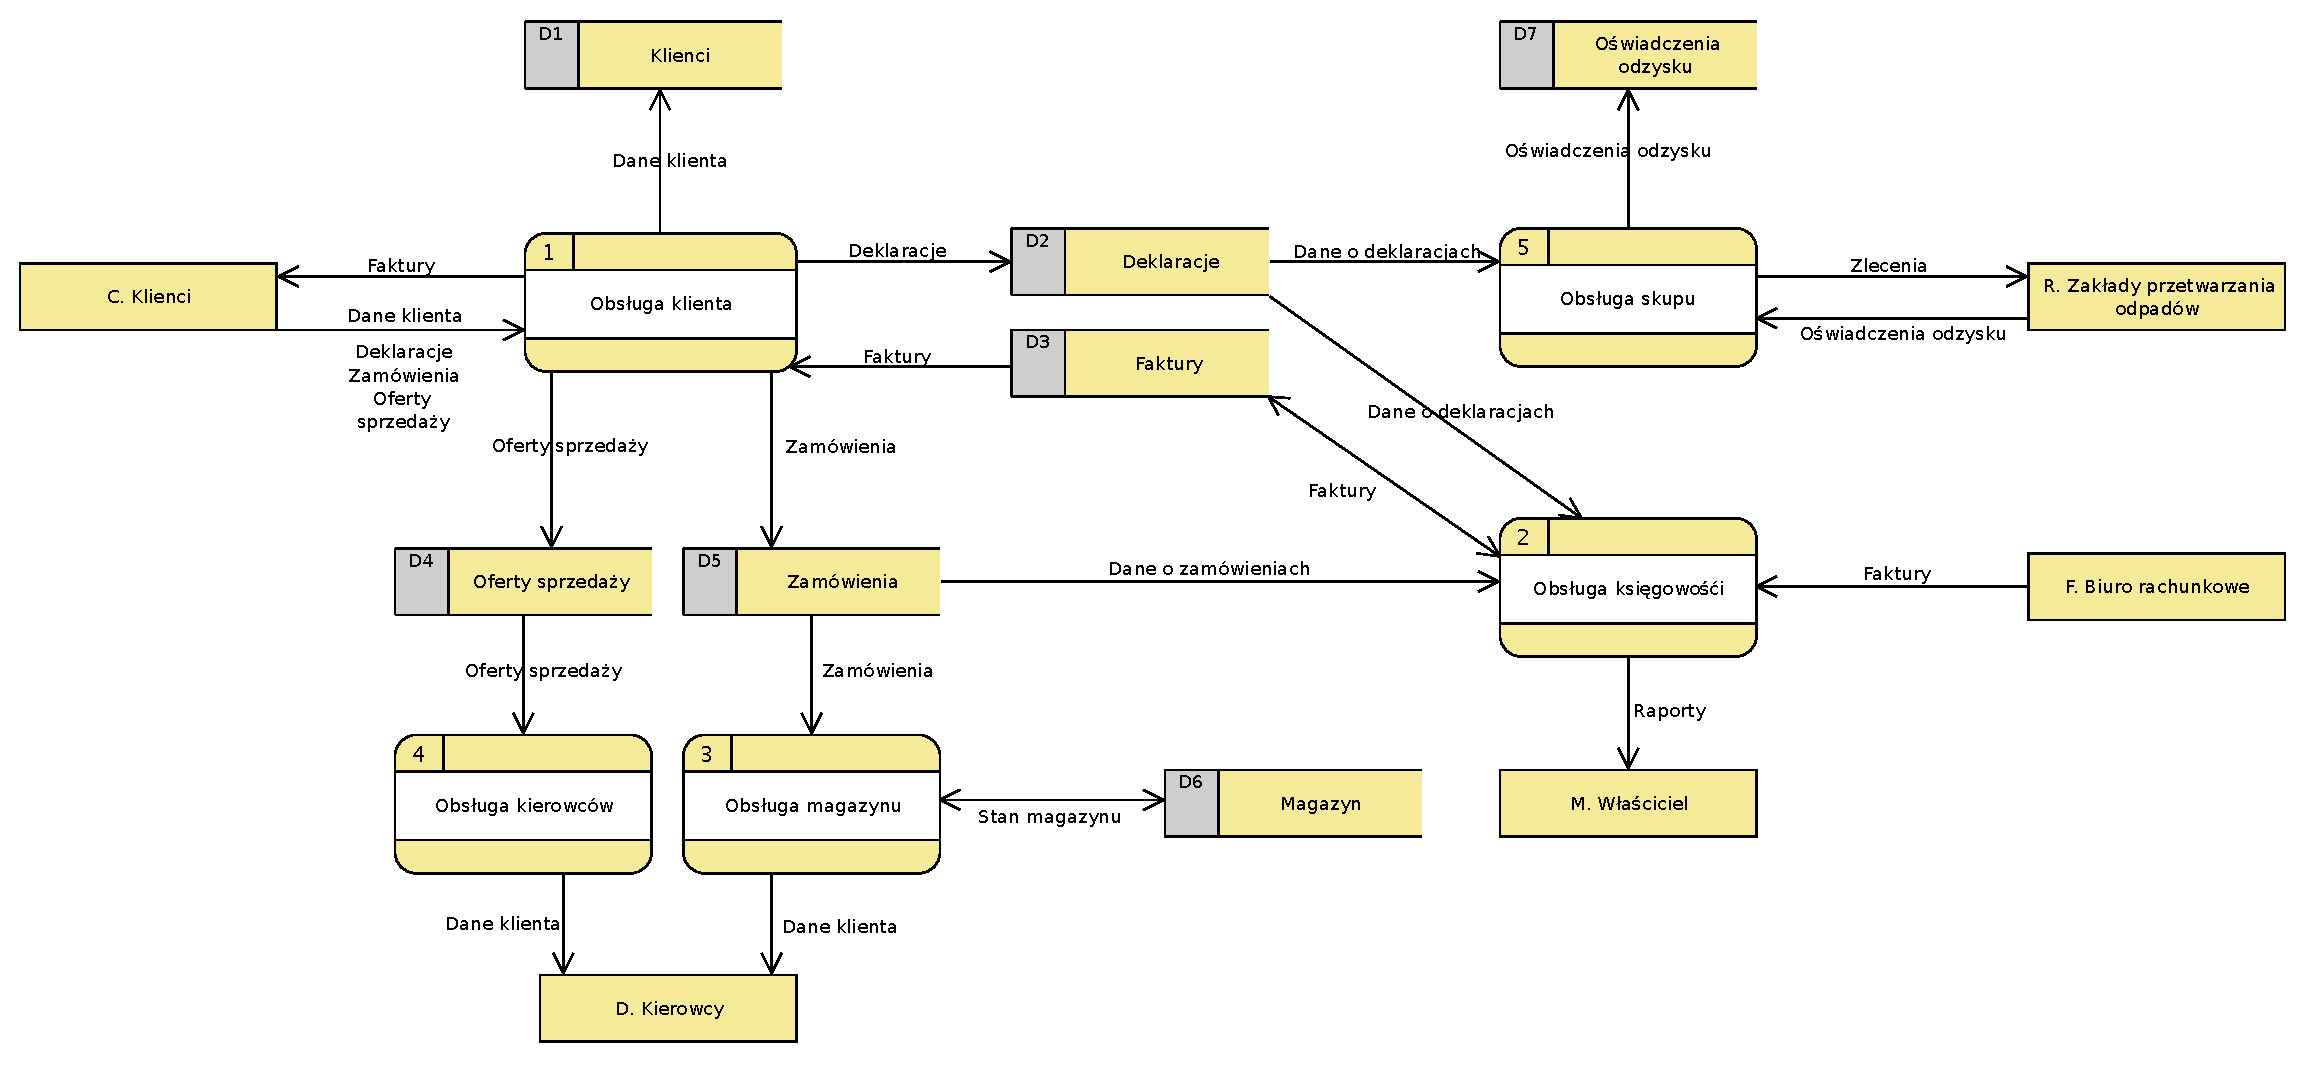
\includegraphics[angle=90, height=29cm]{img/DFD/1-level.eps}}
	%\includepdf[pages={1}, angle=90]{img/DFD/1-level-eps-converted-to.pdf}
\end{figure}

\linespread{1.6}

%DFD1
\textbf{Opis}\\
Digram pokazuje wyodrębnienie podsystemów, które są przedstawione bardziej szczegółowo na kolejnych diagramach.


%DFD3 - Obsługa magazynu
\begin{figure}[H]
	\centering
	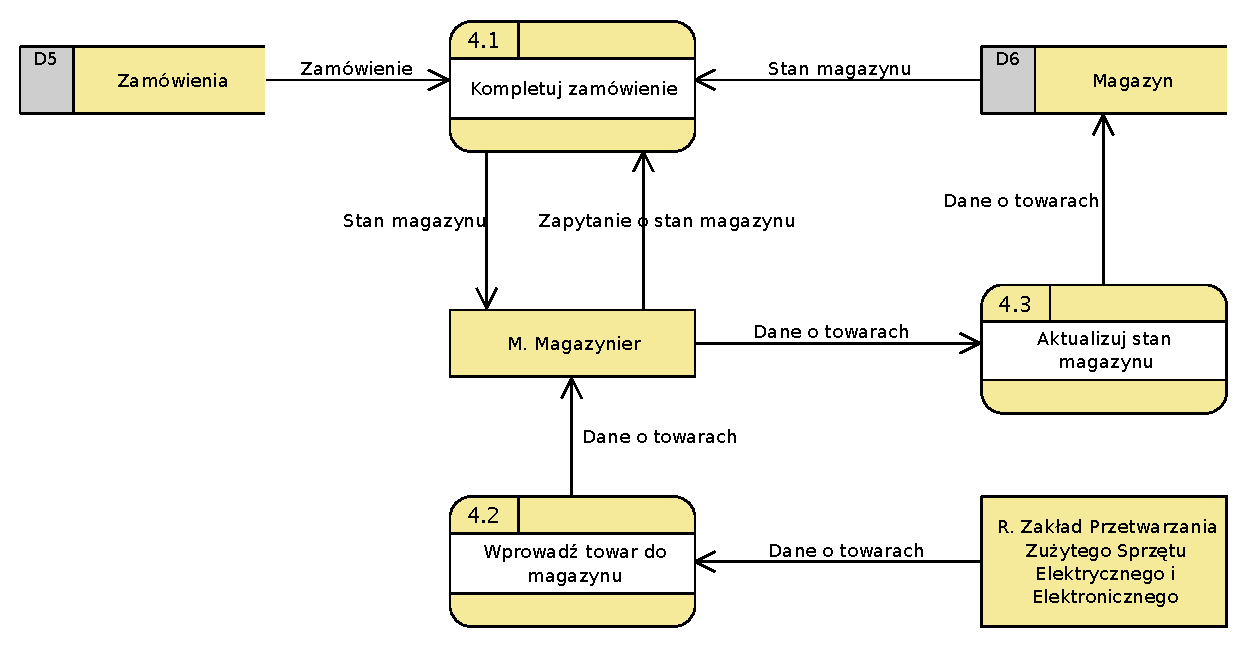
\includegraphics[width=\textwidth]{img/DFD/2-level-magazyn.eps}
\end{figure}

\textbf{Opis} \\
\underline{3.1 Kompletuj zamówienie}\\
Magazynier pyta o stan magazynu, aby sprawdzić, czy może skompletować zamówienie.
\textbf{Strumień wejściowy} zapytanie o stan magazynu, zamówienie\\
\textbf{Strumień wyjściowy} aktualny stan magazynu\\

\underline{3.2 Aktualizuj stan magazynu}\\ 
Stan magazynu jest aktualizowany na podstawie ilości produktów dostarczanych lub odbieranych.\\	
\textbf{Strumień wejściowy} Produkty przyjmawane do magazynu, produkty wydawane przez magazyn.\\
\textbf{Strumień wyjściowy} Produkty przyjmawane do magazynu, produkty wydawane przez magazyn.\\
\underline{3.3 Wprowadź towar do magazynu}\\
Towar zostaje przywieziony przez kierowcę z Zakładu Przetwarzania Zużytego Sprzętu Elektrycznego i Elektronicznego, informacje o jego ilości są zapisywane do systemu.\\
\textbf{Strumień wejściowy} Dane o przywiezionych towarach\\
\textbf{Strumień wyjściowy} Dane o przywiezionych towarach

\begin{figure}[H]
	\centering
	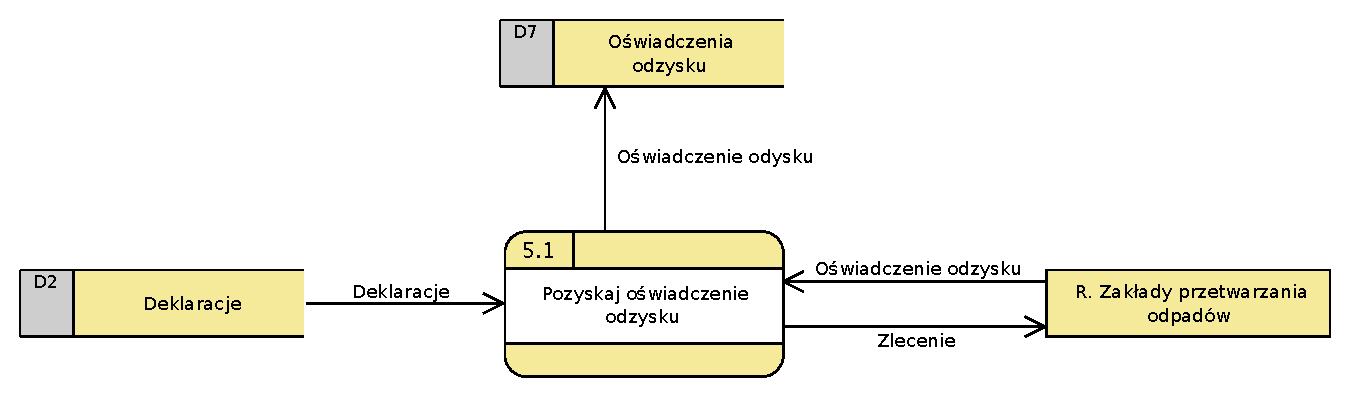
\includegraphics[width=\textwidth]{img/DFD/2-level-skup.eps}
\end{figure}